\pagestyle{myheadings}
\markboth{Astrometry}{Astrometry}
\renewcommand\baselinestretch{1.0}
\setcounter{page}{1}
\begin{center}
{\Huge \bf Astrometry}
\end{center}

Astrometry is the determination of accurate spherical coordinates
($\alpha, \delta$) for an object whose position was previously either 
unknown or poorly established. As well as simply establishing the
position of astronomical sources, astrometry can be used to measure the
proper motion of objects such as asteroids or `nearby' stars, provided
astronomical images at suitably different  epochs are available. 

In fact, 
asteroids move sufficiently quickly that they produce a trail across a
a long exposure CCD image. Measurement of the length of this trail can thus be used to establish 
the proper motion of the asteroid.

The aim of this exercise is to measure the proper motion of the
\setcounter{page}{1}13th-magnitude asteroid (595) Polyxena from its trailed 
image on a 90-minute CCD exposure and hence to estimate its orbital radius from the sun.

{\bf 1.} The position of the beginning and end of the asteroid trail needs to
be established by setting up a coordinate frame (known as a plate solution) fitted to the measured
$x,y$ positions of stars of known RA and Dec which can be seen on the
CCD image around the position of Polyxena. The first thing you
therefore need to do is to load the {\tt polyxena.fits} CCD image into {\sc gaia} and
measure the $x,y$ coordinates of the 25 stars shown in Fig. 6. The stars are numbered, and their 
equatorial coordinates are provided in Table 1, so make
sure you note down which $x,y$ coordinate refers to which star. 

{\bf 2.} You should now have all the information necessary to make a final list 
containing 5 columns: star number, RA, Dec, x, y. Based on this list you can now use {\sc gaia} 
to perform the coordinate transformation (ask your demonstrator to help with this).
Using the grid of 25 
stars, it should be possible to produce a plate solution with a rms of $\simeq 0.5$ arcseconds. When you 
have an good solution, accept the fit and save the {\tt polyxena.fits} image under a 
new filename (e.g. {\tt polyxena-astrom.fits}). Reload 
this new image into {\sc gaia} and carefully measure the (RA, Dec) coordinates of the start and end of the 
asteroid trail (which can be seen near the centre of the field of view).

{\bf 3.} Based on the coordinates of the start and end of the asteroid trail (and the 90 minute 
exposure time), it is now possible to calculate the angular velocity of the asteroid
({\bf think about the cos(Dec) factor!}). Assuming
circular motion for the asteroid's orbital path around the Sun, and
knowing that the field was close to opposition at the time of
observation (see diagram), compute its distance from the Sun in Astronomical Units. 
As indicated by the diagram, you can assume that
the asteroid is orbiting the Sun in the same direction as the Earth.
\begin{figure}
\centerline{\psfig{file=stars.ps,width=18.0cm,angle=0}}
\caption{Screenshot of the polyxena.fits image showing the locations of the 25 stars which can be used to
define the equatorial coordinate system.}
\end{figure}

\newpage
\vspace*{1cm}


\begin{center}
\centerline{\psfig{file=ap3labasteroid.ps,width=16.0cm,angle=0}}
\end{center}

\begin{table}
\begin{center}
\begin{tabular}{|r|l|l|}
\hline
  \multicolumn{1}{|c|}{Star} &
  \multicolumn{1}{c|}{RA} &
  \multicolumn{1}{c|}{Dec} \\
\hline
  1 & 14:52:49.429 & $-$28:54:51.13\\
  2 & 14:52:40.927 & $-$28:56:37.55\\
  3 & 14:51:52.970 & $-$28:58:56.30\\
  4 & 14:51:51.318 & $-$28:59:00.21\\
  5 & 14:52:14.225 & $-$29:02:41.80\\
  6 & 14:52:06.541 & $-$29:03:31.15\\
  7 & 14:51:44.912 & $-$29:02:41.68\\
  8 & 14:52:02.075 & $-$29:05:46.92\\
  9 & 14:52:05.628 & $-$29:11:02.29\\
  10 & 14:52:02.219 & $-$29:12:39.20\\
  11 & 14:52:35.570 & $-$29:09:41.13\\
  12 & 14:53:04.314 & $-$29:05:43.35\\
  13 & 14:53:07.746 & $-$29:04:42.56\\
  14 & 14:51:00.138 & $-$28:58:57.20\\
  15 & 14:50:53.009 & $-$29:00:13.11\\
  16 & 14:51:07.926 & $-$29:12:56.19\\
  17 & 14:52:56.981 & $-$28:59:47.82\\
  18 & 14:52:50.848 & $-$29:01:58.89\\
  19 & 14:52:48.953 & $-$29:03:11.91\\
  20 & 14:52:44.232 & $-$29:03:59.56\\
  21 & 14:52:42.356 & $-$29:05:36.85\\
  22 & 14:51:25.420 & $-$29:08:48.12\\
  23 & 14:51:16.278 & $-$29:06:31.77\\
  24 & 14:51:10.221 & $-$29:08:07.60\\
  25 & 14:51:07.936 & $-$29:06:44.75\\
\hline\end{tabular}
\caption{List of equatorial coordinates for the 25 stars highlighted in Fig. 6}
\end{center}
\end{table}

%\vspace*{2cm}
%{\bf Data for the film/plate used}:\\
%UKST original plate J1494, Field 448, centre 14$^h$ 57$^m\:\: -30^{\circ}$\\
%Plate scale: 67.12 arcsec per mm\\
%Date of observation: 1975 May 17, LST at start of exposure 14$^h$ 46$^m$\\
%Exposure duration: 90$^m$
%RA of Sun on May 17: 3$^h$ 33$^m$\\

%{\bf See}:\\
%KOWAL: Asteroids, their Nature and Utilization (ROE Library
%523.44(02.063))\\
%Ephemerides of Minor Planets 1975 (ROE Library).
